\documentclass[report.tex]{subfiles}
\begin{document}
\subsection{Methodology}
This section is divided into four parts where the fist part describes how to calculate the microstrip parameters used in REF and REF, the second part how to find the signal propagation delay, the third how to analyse SWR and the fourth part analysis of transmission line loads.
\subsubsection{Microstrip Parameters}
The microstrip defined in \ref{subsubsec: Microstrip_Parameters} was simulated in ADS by using the components MLIN and MSUB from the TLines-Microstrip library. The parameters given in \ref{table: Lab1 Microstrip parameters} and the phase shift given in \ref{subsubsec: Lab1 Phase Shift} was entered into the substrate component directly in the schematic and into the transmission line in the LineCalc utility. The conductivity was set to 5.8E7 to represent copper and the thickness of the microstrip was set to 18 $\mu$m. In LineCalc were the width, length and the effective dielectric constant calculated by using the Synthesize commando. The wavelength was calculated by setting the phase shift to 360 $^\circ$ and reading the length of the transmission line. In LineCalc is the phase shift denoted as E\_eff and the effective dielectric constant given as K\_Eff. The result of this operation is given in Table \ref{table: Lab1 Simulated Microstrip parameters}.

\begin{table}[H]
    \centering
    \caption{Simulated microstrip parameters.\label{table: Lab1 Simulated Microstrip parameters}}
    \begin{tabular}{c | c | c | c}
        $w [\text{mm}]$ & $l [\text{mm}]$ & $\epsilon_{eff}$ & $\lambda [\text{mm}]$\\
        \hline
		2.38 & 149.83 & 1.89 & 217.7
    \end{tabular}
\end{table}

\subsubsection{Signal Propagation Delay}
The signal propagation delay is an important factor when working with RF networks. When doing operations on multiple signals, like mixing is it important that the signals are not delayed towards each others. To find the signal propagation delay in a transmission line is the following formula used
\begin{equation}
	\Delta t_p = \dfrac{l}{\nu_p}
\end{equation}
where l are the transmission line length and $\nu_p$ propagation speed.

The propagation speed can be determined by analysing transmission lines with different lengths with the LinearStepRespT template in ADS. By measuring the time it takes for the wave to reach the end of the transmission line is it possible to calculate the propagation speed.
\begin{figure}[H]
	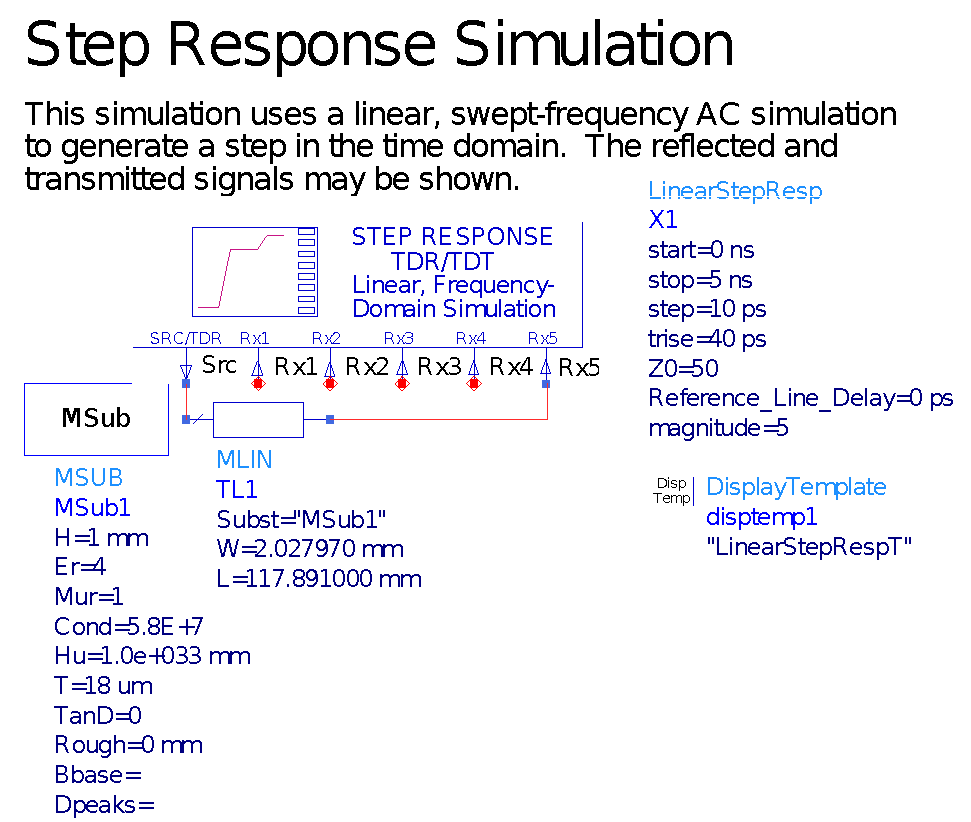
\includegraphics[scale=0.8]{Step_response_setup_2}
	\caption{Setup to measure the propagation speed.}
\end{figure}
In this experiment was the microstrip from section \ref{subsubsec: Microstrip_Parameters} used with the height and relative dielectric constant of the substrate set to 1 mm and 4 respectively and the microstrip parameters was resynthesized.

\subsubsection{Reflection Coefficient}

\begin{figure}
	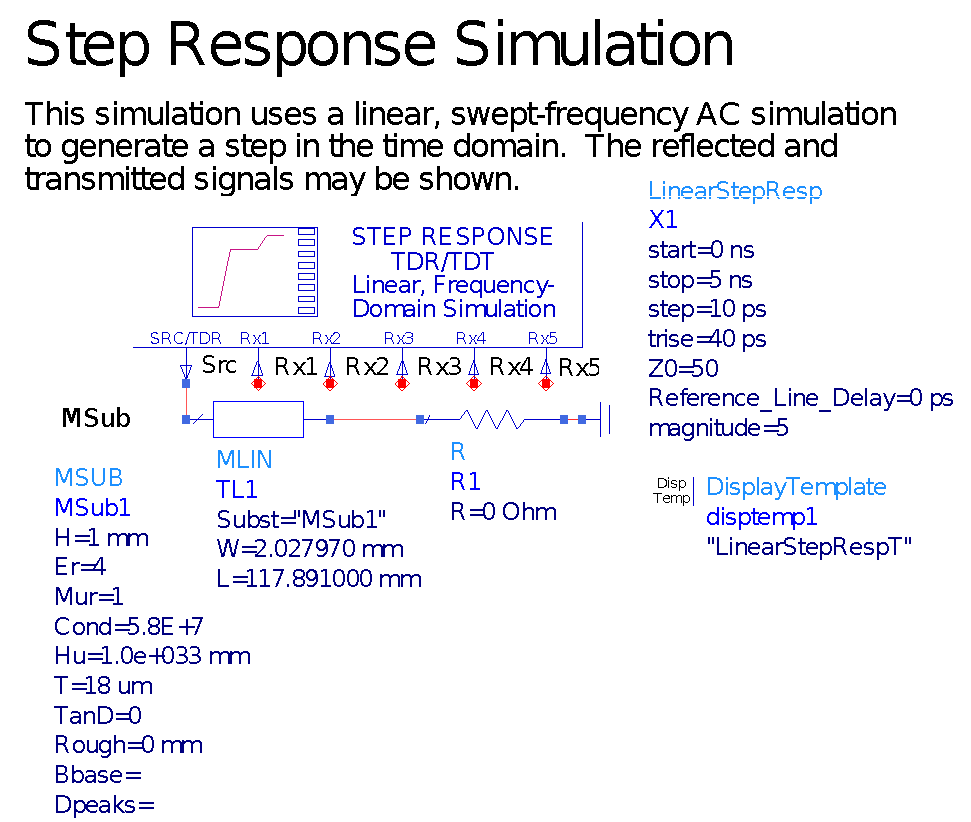
\includegraphics[scale=0.8]{Step_response_setup}[H]
	\caption{Setup to simulate reflection coefficient.}\label{fig:Lab1 reflection coefficient}
\end{figure}

The reflection constant can be simulated by terminating the transmission line with a resistor and analysing the results when sending a pulse with the LinearStepRespT template in ADS. How this looks can be seen in Figure \label{fig:Lab1 reflection coefficient}. By varying the load will different reflection coefficient be the result.

\subsubsection{Transmission Line as Load}
A transmission line has a periodic impedance behaviour where the transmission line represents inductive behaviour in the range of $\left] \dfrac{n}{2} - \dfrac{2n + 1}{4} \right]\lambda$ and with capacitive behaviour in the range of $\left]\dfrac{2n + 1}{4} - \dfrac{1 + n}{2} \right]\lambda$ where n is an integer.

In this experiment was the behaviour of having loads of transmission lines with the lengths of $\lambda$, $\sfrac{\lambda}{4}$ and $\sfrac{\lambda}{8}$ analysed. This with the help of the ADS LinearPulseRespT template.
\end{document}